\section{Method selection and architecture}

\begin{frame}{Convolutional neural network and initial architecture}
\textbf{Method selection}
\begin{itemize}
\item Speed prediction is a \textbf{non-linear regression} task $\rightsquigarrow$ Neural network
\item Use convolution layers to perform feature extraction $\rightsquigarrow$ \textbf{convolutional neural network} (CNN)
\end{itemize}
\textbf{Initial architecture}
\begin{itemize}
\item Paper of NVIDIA work group \cite{NVIDIA2016} of a CNN for self-driving cars
\item Enough complexity and layers to handle the task and lots of possibilities to fine-tune it
\item Initial results with the raw model: MSE of under 3 on the training set and around 18-20 on the testing set\\
$\Rightarrow$ Improvements needed
\end{itemize}
\end{frame}

\begin{frame}[plain]
\begin{figure}
\centering
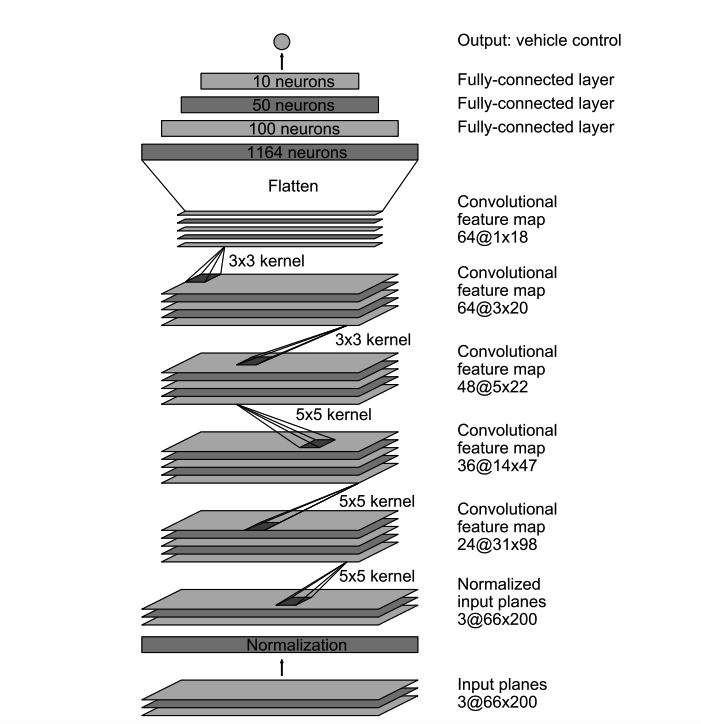
\includegraphics[scale=0.3]{./imgs/NetworkOriginal.png}
\caption{Original architecture of the NVIDIA paper \cite{NVIDIA2016}.}
\end{figure}
\end{frame}